\section{Auswertung}
\label{sec:Auswertung}

% Fehlerrechnung
Die in diesem Kapitel durchgeführten Fehlerrechnungen wurden mittels der Gaußschen Fehlerfortpflanzung 
\begin{equation}
    \sigma_f = \sqrt{\left( \frac{\partial f}{\partial x_1} \sigma_{x_1} \right)^2 + \left( \frac{\partial f}{\partial x_2} \sigma_{x_2} \right)^2 + ...}
\end{equation}
durchgeführt, sowie den Formeln 
\begin{equation}
    \overline{x} = \frac{1}{n} \sum^n_{i=1}x_i . 
    \label{eq:mittelwert}
\end{equation}
für den Mittelwert und 
\begin{equation}
    \sigma_{\overline{x}} = \frac{\sigma_x}{\sqrt{n}} = \sqrt{\frac{1}{n(n-1)}  \sum^n_{i=1} \left( x_i - \overline{x}\right)^2 } .
    \label{eq:abweichung}
\end{equation}
für die Standardabweichung einer Messreihe $\left( x_1, ... , x_n  \right)$.
Der Einfachheit halber wird hierbei das Python-Paket \textit{uncertainties} verwendet. \cite{uncertainties} \\
\hspace{1cm}
% Ende Fehlerrechnung

\subsection{Justieren der Verzögerungsleitung}
\begin{figure}[H]
    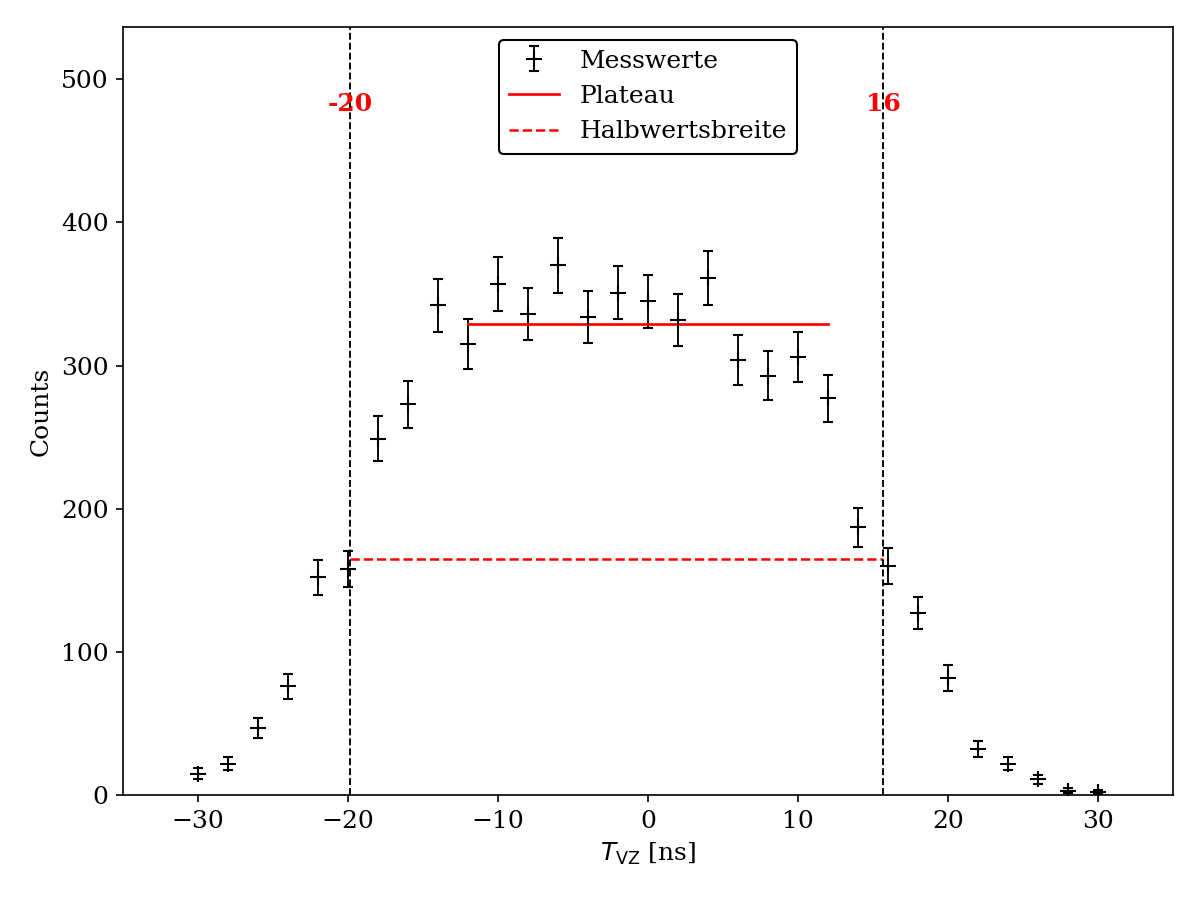
\includegraphics[width=0.7\textwidth]{v01/content/plots/delay_plot.png}
    \caption{Justierung der Verzögerungsleitung.}
    \label{fig:delay}
\end{figure}
\subsection{Bestimmung der Channelzuordnung}
In der ... sind die Messwerte zur Bestimmung der Channelzuordnung dargestellt. 

\begin{table}[H]
    \centering
    \caption{Kalibrationsdaten des Vielkanalanalysators (MCA).}
    \label{tab:mca_kalibration}
    \begin{tabular}{S[table-format=1.1] S[table-format=3.2]}
        \toprule
        {$t \: / \: \unit{\micro\second}$} & {Kanal-Nr.} \\
        \midrule
        0.5 & 16.27 \\
        1.0 & 39.32 \\
        1.5 & 62.23 \\
        2.0 & 85.02 \\
        2.5 & 108.02 \\
        3.0 & 131.00 \\
        3.5 & 154.02 \\
        4.0 & 177.00 \\
        4.5 & 200.08 \\
        5.0 & 223.10 \\
        5.5 & 246.26 \\
        6.0 & 269.31 \\
        6.5 & 292.83 \\
        7.0 & 315.93 \\
        7.5 & 338.96 \\
        8.0 & 361.98 \\
        8.5 & 385.00 \\
        9.0 & 408.00 \\
        9.5 & 431.00 \\
        9.9 & 449.17 \\
        \bottomrule
    \end{tabular}
\end{table}
Daraus ergibt sich die lineare Regression der Form
\begin{equation*}
    t(K) = a \cdot K + b, 
\end{equation*}
mit den Parametern
\begin{align*}
    a &= \qty{0.045(0.001)}{\micro\second} \\
    b &= \qty{0.18(0.05)}{\micro\second} \,.
\end{align*}
Daraus lassen sich die Zeiten den Kanälen zuordnen, wie in \autoref{fig:channel} dargestellt. 
\begin{figure}[H]
    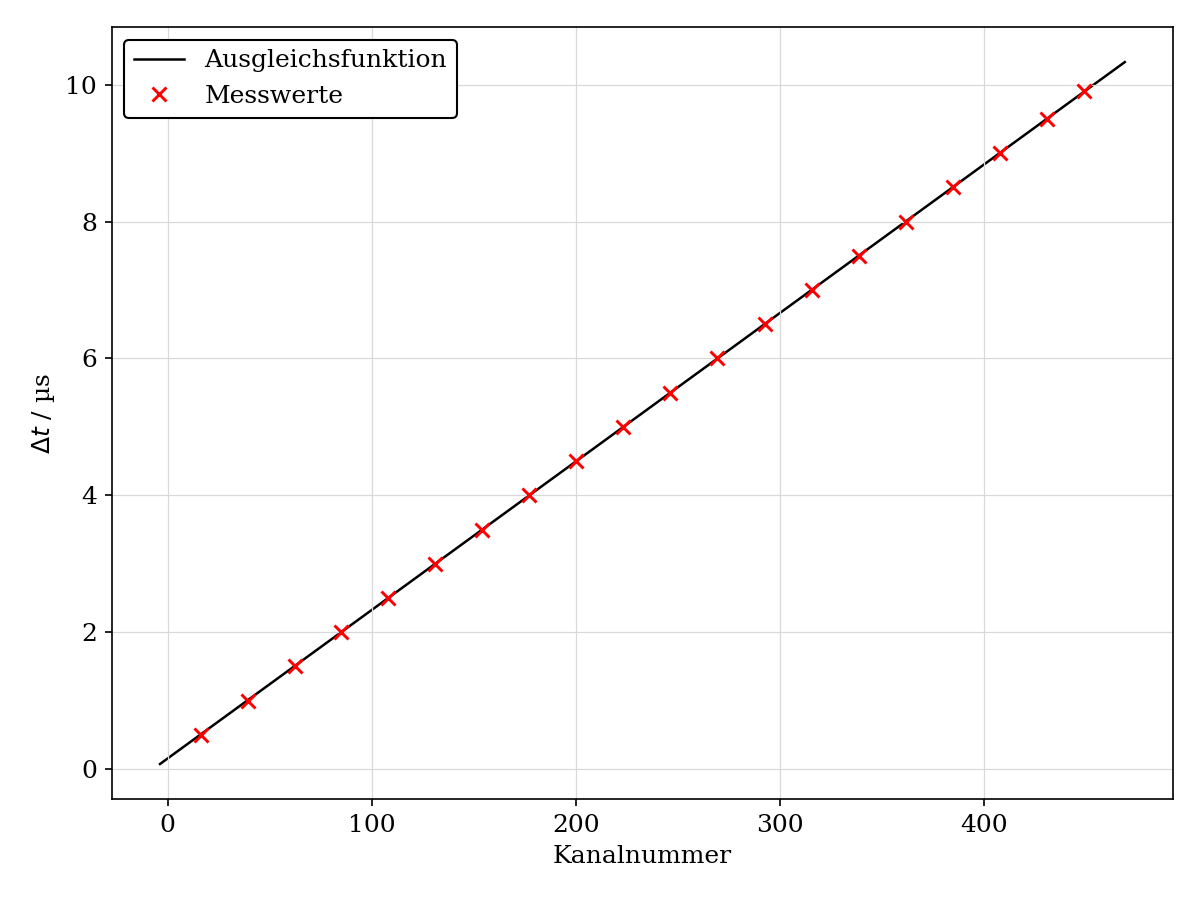
\includegraphics[width=0.7\textwidth]{v01/content/plots/channel_plot.png}
    \caption{Bestimmung der Channelzuordnung.}
    \label{fig:channel}
\end{figure}
\subsection{Bestimmung der Lebenszeit}
Es wurde über einen Zeitraum von $t = \qty{258769}{s}$ gemessen, hierbei wurden ungefähr $N_{\text{Start}} = 986743$ Startsignale aufgenommen und $N_{\text{Stopp}} = 813$ Stoppsignale aufgenommen.
Dazu ist anzumerken, dass beim Ablesen der Start- und Stoppsignale der Zähler Startsignale nicht weiter anstieg, der Zähler der Stoppsignale hingegen schon.
Es wurden $N_{\text{gefüllt}= 466}$ Kanäle gefüllt.
\begin{figure}[H]
    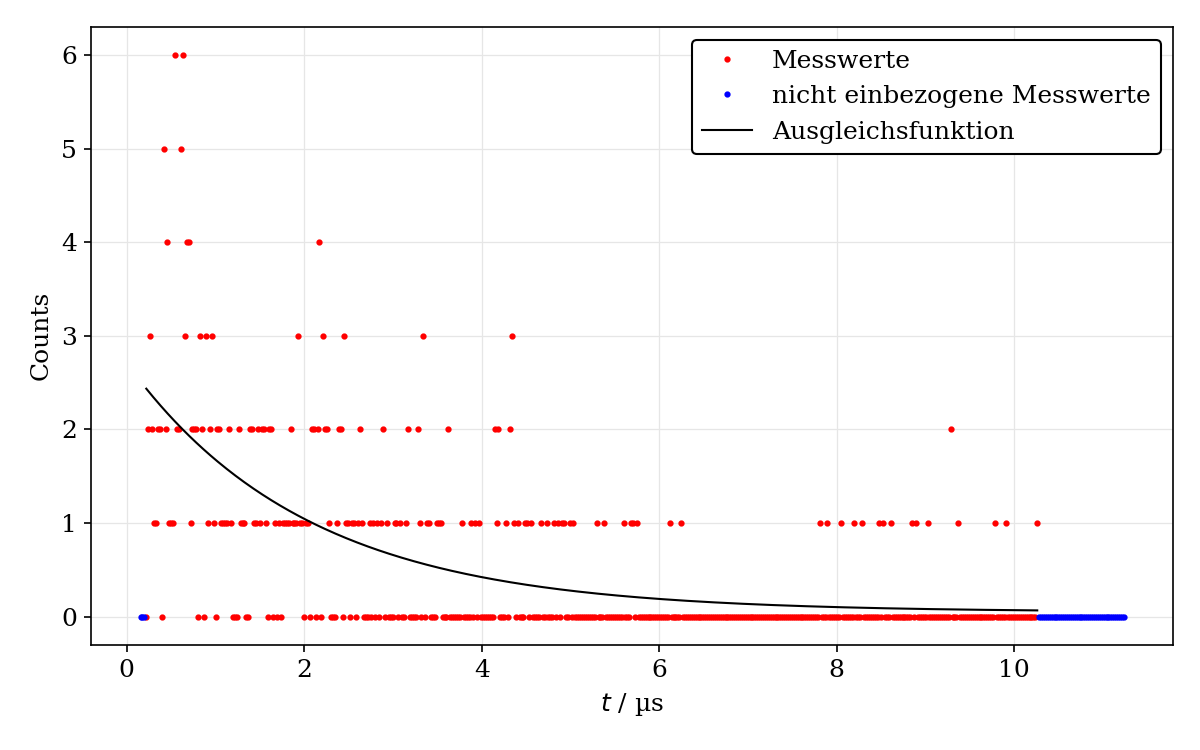
\includegraphics[width=0.7\textwidth]{v01/content/plots/lifetime_plot.png}
    \caption{Lebenszeitverteilung der Myonen.}
    \label{fig:lebenszeit}
\end{figure}
Hierbei wurden die Kanäle von 20 bis 450 betrachtet, da die Kanäle unterhalb von 20 nicht gefüllt waren und die Kanäle oberhalb von 450 nur wenige Einträge hatten.
Mithilfe der exponenziellen Regression der Form
\begin{equation*}
    N(t) = N_0 \exp \left( -{\lambda t} \right) + U
\end{equation*} 
folgt für die Parameter:
\begin{align*}
    N_0     &= \num{2.66(0.18)} \\
    \lambda &= \qty{0.49(0.07)}{\per\micro\second} \\
    U       &= \num{0.05(0.07)} \,.
\end{align*}
Die Lebenszeit der Myonen berechnet sich über die Formel
\begin{equation*}
    \tau = \frac{1}{\lambda},
\end{equation*}
woraus sich für die Lebenszeit der Myonen $\tau = \qty{2.04(0.28)}{\micro\second}$ ergibt.

\subsection{Bestimmung der Untergundrate}

\clearpage